\documentclass[10pt,a4paper]{article}
\usepackage[latin1]{inputenc}
\usepackage{amsmath}
\usepackage{amsfonts}
\usepackage{amssymb}
\usepackage{graphicx}
\usepackage{soul}
\usepackage{caption}
\usepackage{subcaption}
\usepackage[left=2cm,right=2cm,top=2cm,bottom=2cm]{geometry}
\author{Akshat Mahajan}
\title{Physics 180Q - Lab Report 2}
\begin{document}
\maketitle

\textsl{This lab was performed in conjunction with Hanwen Qin. The variable impedance terminator was set to 10 k$\Omega$ throughout, as analysis of the results from Week 1 had demonstrated that it gave the most accurate responses overall.}

\section*{Part 1: Crossed Polarizers}

We took two polarisers and used them to obtain a vertical polariser in series with a horizontal polariser (i.e. in the crossed state). We decided to orient the first polariser parallel to the polarisation of the light, and then to simply orient the second axis until an aligned (maximum throughput power) and crossed state (minimum throughput power)  was achieved. Not initially knowing what the transmission axes of the polarisers were (we only later discovered the red mark that signifies the transmission axes on the back of the polariser), we simply measured the power through the first polariser until it came to a maximum to determine when it was perfectly aligned with the incoming light. This was achieved at an angle of 112$^{\circ}$ from the vertical for the first polariser. The crossed state was found to occur when the second polariser was at 10$^{\circ}$, and the aligned state at 280$^{\circ}$ (exactly ninety degrees to the left of our crossed state).\\
\\
Afterwards, we inserted a third polariser while the other two were in their crossed state, and measured the power through this system as a function of angle. Unfortunately, we did not measure the transmission axis of the polariser itself, so all of our results will be offset by some unknown phase shift.\\ 
\\
The background correction for light impinging on the detector was found to be 300 $\mu$V with the lights off, and 5.3 $\pm$ 3 mV with the lights on.

\begin{enumerate}
\item What is the residual transmission in the crossed state, and what is the transmission when the two polarizers are aligned? What is the extinction ratio? 

\textbf{Answer:} The voltage through the crossed state was found to be \textbf{300 $\pm$ 200$\mu$V} (1 $\times$ 10$^{-4}$ mW) with the lights off. The voltage through the aligned state was found to be \textbf{1.16 V (0.3 mW)} with the lights off (for reference, the light entering through the first polariser was found to be 1.40 V (0.46 mW)).

Transmission through the crossed state $\approx$ 0\%.Transmission through the algined state $\approx$ 82\%. The extinction ratio is 10 log $\left(\dfrac{P_{y}}{P_{x}}\right) = $ 10 log $\left(\dfrac{1.16}{300 \times 10^{-6}}\right)= 35.8 $. 

\item With the two polarizers in the crossed state, insert another polarizer between them and plot the transmission of the system as you rotate the central polarizer.

\textbf{Answer:} See Figure 1 below. No phase correction has been made.

\item How does this compare with the result of the prelab?

\textbf{Answer:} \ul{They correspond almost exactly}. The form of the electric field is proportional to $\sin(2\theta)$, so that the power is then just $\sin^{2}(2\theta)$. Figure 1 demonstrates how the theoretical prediction (right panel) correlates with the experimental value (left panel). One can see at once that they match nearly perfectly; that there is an unaccounted for phase difference between the left and right panels; and that there is only one note of discrepancy, namely the uneven heights. This can be attributed to systematic error, namely that not all of the light appears to have been falling on the photodetector. There is also a near constant offset, which can be attributed to background noise.
\end{enumerate}
\begin{figure}[h]
\centering
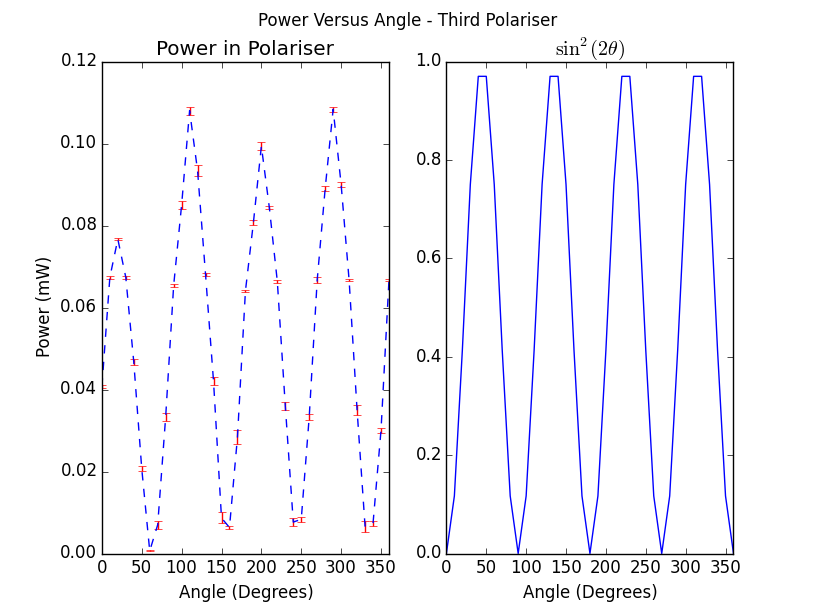
\includegraphics[scale = 0.6]{../Analysis/figure_1.png}
\caption{Figure Relevant to Part 1. Right panel corresponds to experimental observation; left corresponds to theory. Red bars on the left panel are error bars. Height on left panel is without units.} 
\end{figure}
\section*{Part 2: The Behaviour of Waveplates}
In this section, we attempted to characterise the behaviour of waveplates using two polarising beam splitters and (of course) a waveplate. In the absence of two photo-diodes, we were content to measure the initial total power prior to entering the second beam splitter, and then measuring the power through one arm of the beam. The power through the second arm of the beam was determined by subtracting the power through the first arm from the power through the PBS. The total voltage\footnote{Partway through the experiment, the table was actually knocked slightly, disturbing the setup. At the time, not having plotting software on us, we did not think the difference following it was large enough to merit redoing the  experiment. This is one source of error in our setup. After this point, however, the power was not changed.} was measured to be 1.91 V (0.63 mW). A half-wave plate was inserted just before the second polarising beam splitter, and was varied in ten degree increments over 360 degrees. As before, no attempt was made to ascertain the transmission axis prior to measurement, so results will be offset by some constant phase.

\begin{enumerate}
\item Rotate the HWP in 10 degree increments and record the power in both arms of the PBS. Compare this to theory (using e.g. the Jones matrices techniques).

\textbf{Answer: } See Figure 2 below. The Jones matrix approach predicts a $\sin^{2}\left(2\theta\right)$ behaviour for the power distribution through one arm, and a $\cos^{2}\left(2\theta\right)$ behaviour through the other. The experimental observations - barring a phase difference - match up almost perfectly with theory.
\begin{figure}[t!]
\centering
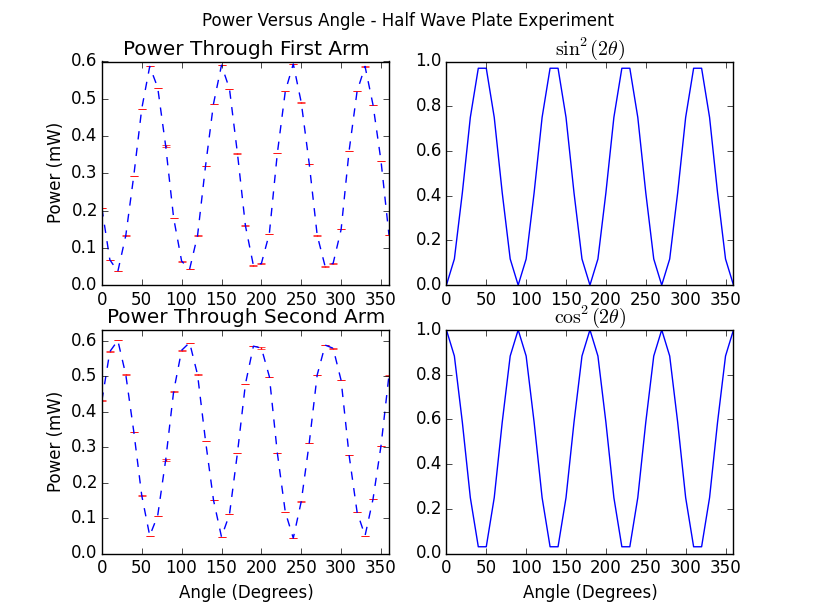
\includegraphics[scale = 0.6]{../Analysis/figure_2.png}
\caption{Figure Relevant to Part 2, Question 1. Red bars on the left panels are error bars. Height on left panels is without units.} 
\end{figure}
\item Can you distinguish which one is the fast axis and which one is the slow? If not, try to think of a trick to do this.

\textbf{Answer: } \ul{No, I cannot distinguish between the slow or fast axis}. Even in theory, the half-wave plate does little but to introduce a negative sign in front of the amplitude in a particular direction; on squaring, the worked power turns out to be the same as before. In our experimental setup, we're also creating equal amplitude coefficients that differ only with whether or not they're multiplied by a cosine or a sine. Distinguishing which one is leading and by what factor is not possible in this setup.

\item Insert a mounted QWP between the two polarizers. Rotate the QWP in 10-degree increments and record the power in both arms of the PBS. Compare this to theory (using e.g. the Jones matrices techniques).

\textbf{Answer: } See Figure 3. For the most part, they agree well. Although the Jones matrix method predicts a $\cos^{2}(\theta) - i\sin^{2}(\theta)$ distribution for power, squaring these quantities results in a similar $\cos^{2}(2\theta)$ power distribution as before. Once again, we did not note the transmission axis of the quarter-wave plate prior to performing this experiment, so some phase difference attributable to the orientation (as opposed to the effect) of the quarter wave plate is inevitable. 
\begin{figure}[b!]
\centering
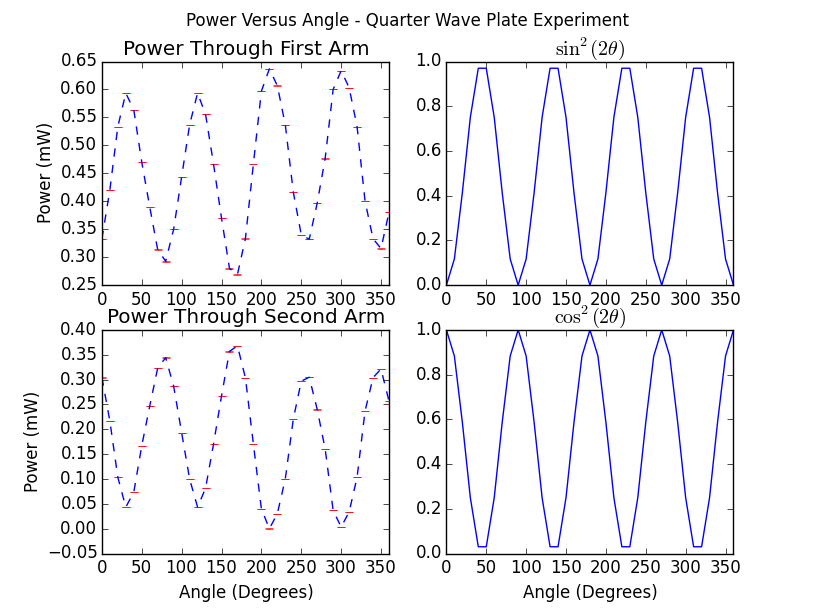
\includegraphics[scale=0.6]{../Analysis/figure_3.png}
\caption{Figure Relevant to Part 2, Question 3. Red bars on the left panels are error bars. Height on left panels is without units.} 
\end{figure}
\item Determine the location of the fast and slow axes. How do you know when the light is circularly polarized?

\textbf{Answer: } The light is circularly polarised when the light through both arms of the PBS are \textsl{equal} - in other words, when the angle of the wave plate is 45$^{\circ}$ to the transmission axis. The fast and slow axes are marked on the wave plate.

\item Can you distinguish which one is the fast and which one is the slow? If not, try to think of a trick to do this.

\textbf{Answer: } Yes, I can determine which one is the fast/slow axis by superimposing a plot of power and angle of the two arms on top of each other. The fast axis always tends to have more power than the other axis because it has the larger coefficient - the phase difference ensures this. This trick won't work for the half-wave plate in our experiment, for reasons outlined in Question 2 of this section - in particular, both arms oscillate over the entire power spectrum in the HWP, whereas one (faster) arm tends to occupy the higher half of the power spectrum while the other (slower) occupies the lower half with the QWP. This is shown graphically in Figure 4.
\begin{figure}[h]
\centering
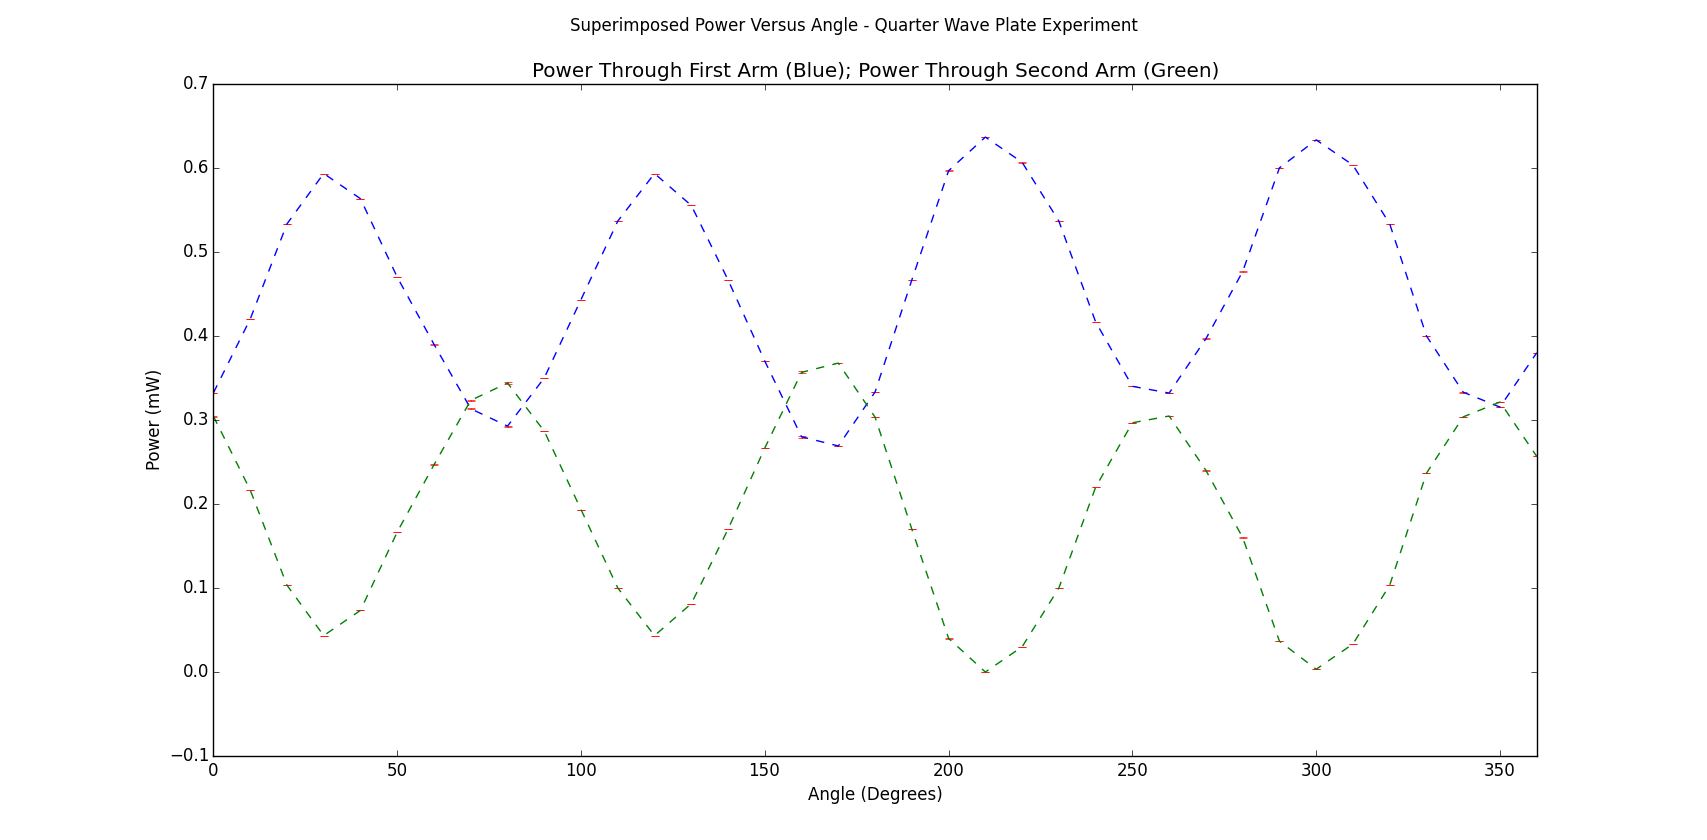
\includegraphics[width = \textwidth]{../Analysis/figure_5.png}
\caption{Figure Relevant to Part 2, Question 5. Red bars are error bars..} 
\end{figure}
\end{enumerate}
\section*{Part 3: Verifying the Creation of Circularly Polarized Light}
We created circularly polarised light by keeping the polariser at 45$^{\circ}$ to the transmission axis. In this case, that meant keeping the QWP plate at 170 degrees to the vertical, where the minimum had occured and where we (in retrospect erroneously) concluded that the light beams would have equal intensity. \textit{We now realise that this is not in fact circularly polarised light, judging from Figure 4. A better candidate would have been 350 degrees, or somewhere where the intensities were equal.}\\
\\
Because we did not know the transmission axis of the HWP, we chose to rotate the HWP in ten-degree increments from 0 to 360 degrees. The error involved in this measure is $\pm$ 10 degrees. In the interests of time, we chose to take advantage of sinusoidal symmetry this time and simply measure upto 180 degrees.
\begin{enumerate}
\item Insert a HWP into your circularly polarized light beam and repeat the measurement of part 2a. Compare the results to theory. Did you make circularly polarized light?

\textbf{Answer: } See Figure 5. Theory predicts a \textsl{constant} power (half of the incoming beam) in both arms of the PBS - in other words, the angle of the HWP should not affect our measurement at all. We do \ul{not} see this in our results, as there is some demonstrated   sinusoidal variation about the half-intensity mark. This leads us to conclude that we did not create circularly polarized light - we chose the wrong angle on the quarter-wave plate. It does appear we were pretty close, though.
\begin{figure}[h]
\centering
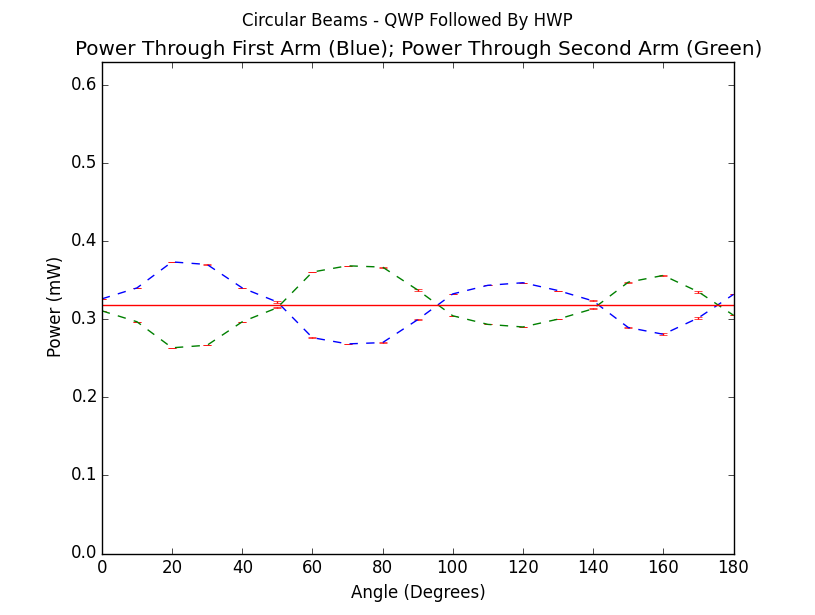
\includegraphics[scale = 0.6]{../Analysis/figure_6.png}
\caption{Figure Relevant to Part 3, Question 1. Red bars are error bars. The red line is our theoretical distribution.} 
\end{figure}
\item Remove the HWP and insert a QWP (use the one with the fast axis labeled) into your circularly polarized light beam. Repeat the measurement of Part 2b. Compare the results to theory. Did you make circular polarized light? Can you identify the handedness of the polarization?

\textbf{Answer: } See Figure 6. It's fairly clear by now that we don't have circularly polarised light. Theory predicts the distribution to be of the order $\cos^{4}(t)$, but I strongly suspect this has been incorrectly calculated. 
\begin{figure}[h]
\centering
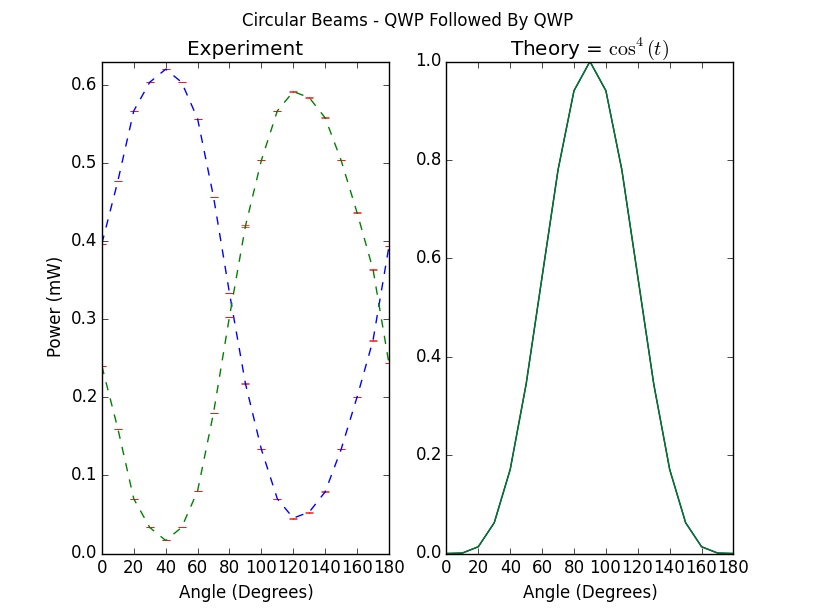
\includegraphics[scale = 0.6]{../Analysis/figure_8.png}
\caption{Figure Relevant to Part 3, Question 2. Red bars are error bars. The blue line indicates power through the first arm; the green line indicates power through the second arm.} 
\end{figure}
\item Slightly rotate the waveplate you used to make the circularly polarized light so that you are now making elliptically polarized light. Redo the measurement of part 3a. Compare the results to theory. What can you say about the polarization you have created?

\textbf{Answer: } See Figure 7. We rotated the QWP so that it was now at 150 degrees instead of 170. This is obviously elliptically polarised light. Compared to our answer in Part 3, Question 1, the variation is much larger. 
\begin{figure}[b]
\centering
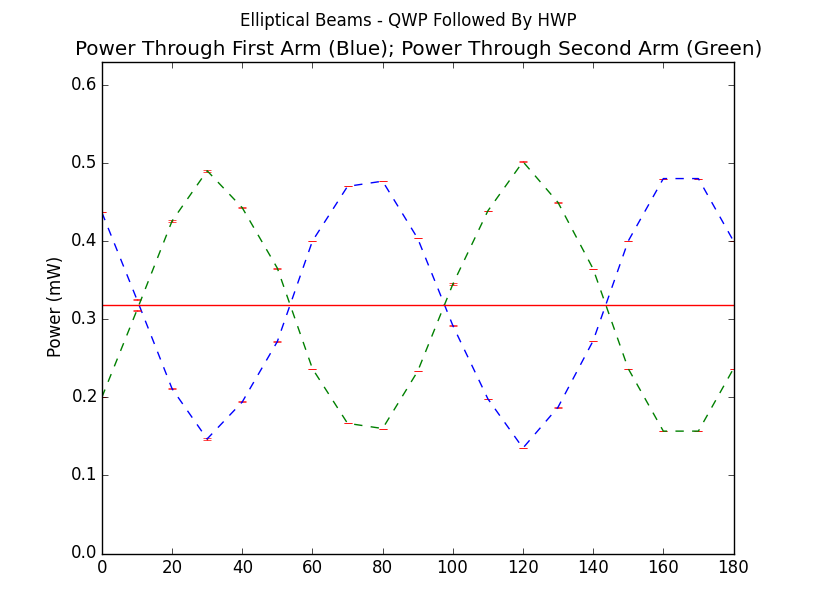
\includegraphics[scale = 0.6]{../Analysis/figure_9.png}
\caption{Figure Relevant to Part 3, Question 3. Red bars are error bars.} 
\end{figure}
\end{enumerate} 
\section*{Part 4: The Poor Man's Optical Isolator}
In this section, we explored ways of preventing back-reflection from propagating through to the system. We built an optical isolator experiment by placing a PBS and QWP in conjunction with each other. A mirror was placed in front of the QWP, reflecting back most of the light. We placed the photodiode on the other side of the PBS. 
\begin{enumerate}
\item Construct the double pass configuration drawn below and measure the power transmitted through the PBS in 10-degree increments on the QWP. Compare to theory and identify which configuration gives the best performance as an optical isolator.

\textbf{Answer :} See Figure 10. We took advantage of sinusoidal symmetry to simply sample up to 180 degrees. We see that some power is lost, so that the total phase is not 0.63 mW - we attribute this to the spreading of the laser beam as it traveled in its path. Our mirror also appeared to be scratched at the back, which may have resulted in some power loss. The maximum power was recorded at about 0.53 mW at 80 degrees. Again, we did not record the axis of transmission of the polariser, so there is a phase difference in our resulting plot. 
\begin{figure}[h]
\centering
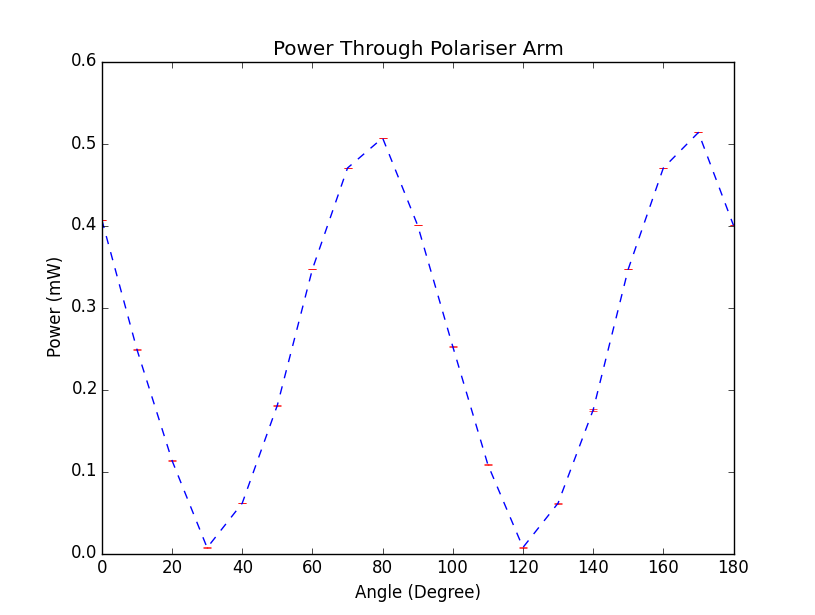
\includegraphics[scale = 0.6]{../Analysis/figure_10.png}
\caption{Figure Relevant to Part 4, Question 1. Red bars are error bars.} 
\end{figure} 
\item This scheme for optical isolation has several significant drawbacks. For example, what would happen if the experiment changed the polarization of the back-­reflected light? How could you improve on this design?

\textbf{Answer: } If the experiment changed the polarisation of the light, then our optical isolator fails: the polarising beam splitter will send some small component back into the laser as the total phase will not have been affected by 90 degrees overall. One simple fix would be to measure the polarisation of the back-reflected light and orient the polariser until the back-reflected component is sufficiently out of phase that the PBS changes its direction. 
\end{enumerate}
\section*{Part 5: Creation of an Arbitrary Polarisation of Light}
\begin{enumerate}
\item Using the results from your Prelab, set up a quarter wave plate and half wave plate to produce light with ellipticity of 0.25 and an orientation of 45 degrees away from vertical. Verify that this is the state of polarization that you obtained. Describe your procedure that demonstrates this.

\textbf{Answer: } To accomplish this, we began by setting an HWP in series with a QWP so that the axes of transmission marked `slow' were aligned together. We knew that we wanted an ellipticity of 0.25, the arctangent of which is 14 degrees. Half of this arctangent is the degree to which we wanted to turn our HWP - so we turned our HWP by a degree of seven. Next, we wanted to observe an angle of 45 degrees in our resulting system, so we rotated our QWP by 45 degrees, and our HWP by an additional 22.5, making our total angle 29.5 on the HWP. Finally, since this works for horizontally polarised light but not for vertically polarised light (which our system consisted of), we rotated both of our systems by 90 degrees (a move that in retrospect was in error - the QWP should have been turned by 180 degrees to preserve the effect). 

To demonstrate our effects, we varied the HWP by 10 degrees and the QWP by 20 degrees to observe the behaviour at different angles. We tried to directly calculate the angle of our polarisation and the ellipticity using trigonometry. In the adjoining table, Column 4 corresponds to our measure of the angle; Column 5 corresponds to our measurement of the ellipticity. We \ul{did not} create elliptical light of our desired proportions, but we did come close.
\end{enumerate}

\begin{table}[h]
\centering
\begin{tabular}{|c|c|c|c|c|c|}
\hline 
QWP Angle & HWP Angle & $P_{x}$ & $P_{y}$ & $\tan^{-1}\left(\dfrac{\sqrt{P_{y}}}{\sqrt{P_{x}}}\right)$ & $\sqrt{P_{y}/P_{x}}$ \\ 
\hline 
347 & 264 & 0.26 mW & 0.37 mW & 0.87 & 0.84 \\
7 & 274 & 0.40 mW & 0.22 mW & 0.63 & 0.74 \\  
27 & 284 & 0.48 mW & 0.14 mW & 0.50 & 0.55 \\ 
\hline 
\end{tabular} 
\end{table}

\begin{figure}
\begin{subfigure}[b]{0.3\textwidth}
\centering
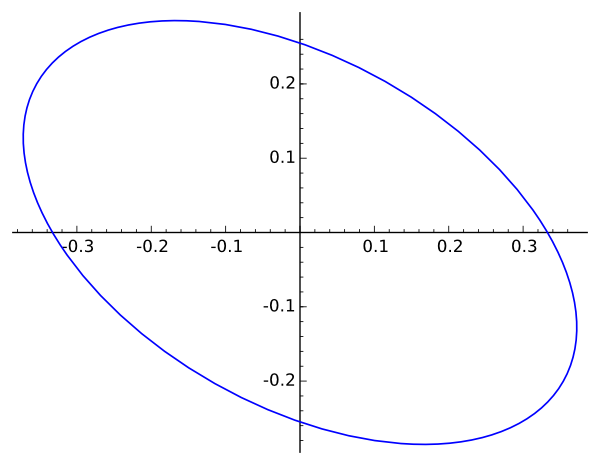
\includegraphics[width=\textwidth]{../Analysis/QWP347.png} 
\caption{QWP = 347$^{\circ}$}
\end{subfigure}
\begin{subfigure}[b]{0.3\textwidth}
\centering
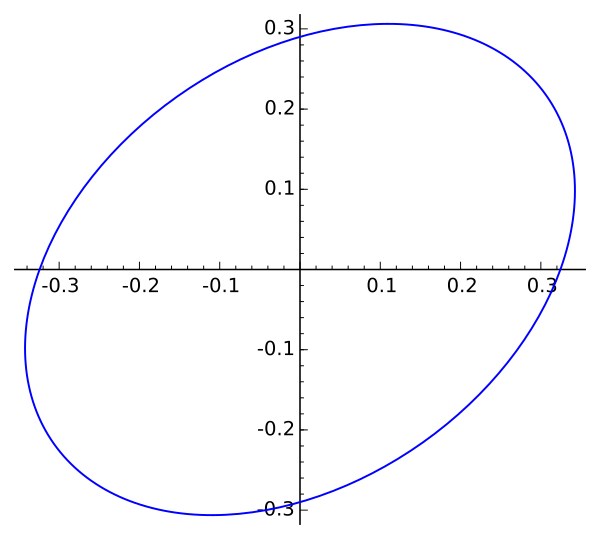
\includegraphics[width=\textwidth]{../Analysis/QWP7.png}
\caption{QWP = 7$^{\circ}$}
\end{subfigure}
\begin{subfigure}[b]{0.3\textwidth}
\centering
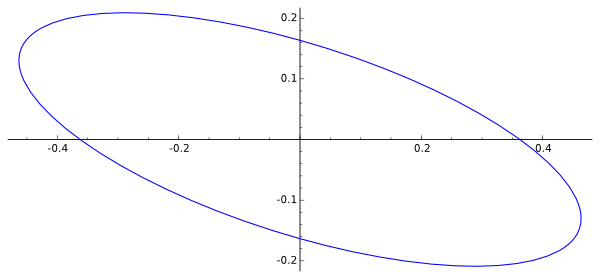
\includegraphics[width=\textwidth]{../Analysis/QWP27.png} 
\caption{QWP = 27$^{\circ}$}
\end{subfigure}
\caption{Figures relevant to Part 5, Question 1}
\end{figure}
\end{document},